\section{Durchführung}
\label{sec:Durchführung}

Bei diesem Versuch wird das sogenannte Sagnac Interferometer untersucht, dessen
schematischer Aufbau in Abbildung \ref{fig:aufbau} dargestellt ist.
\begin{figure}
  \centering
  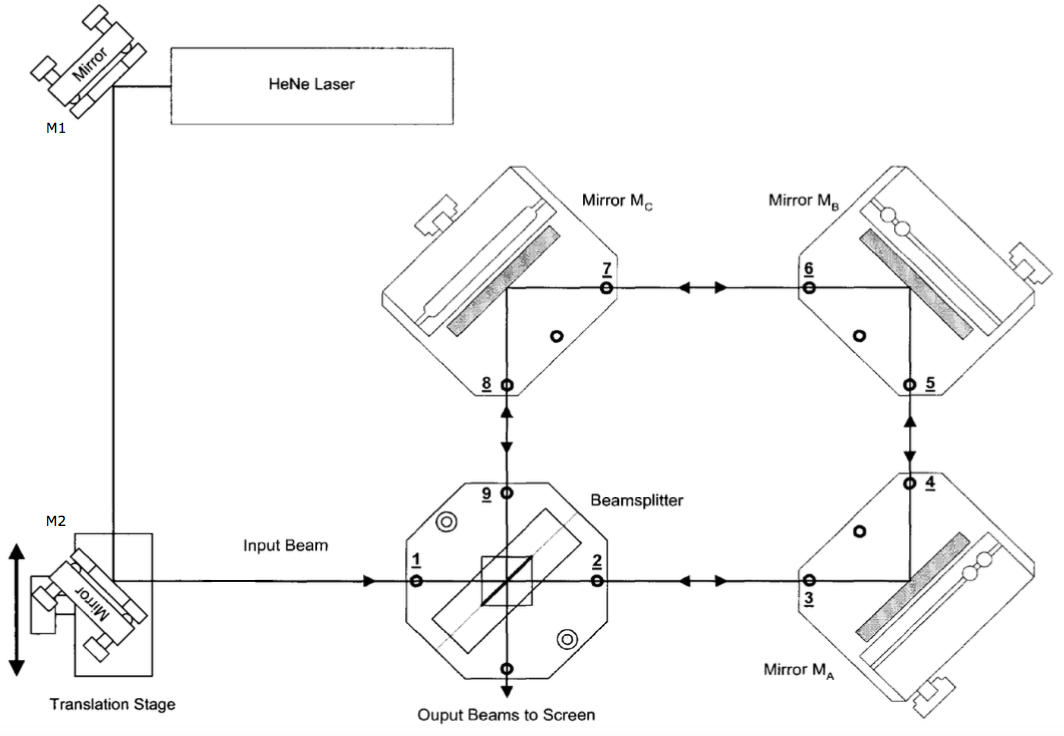
\includegraphics[width=14cm]{Aufbau.png}
  \caption{Schematischer Aufbau eines Sagnac Interferometers \cite{skript}}
  \label{fig:aufbau}
\end{figure}
Die Lichtquelle ist hierbei ein Helium-Neon Laser, welcher linear polarisiertes Licht
mit einer Vakuumwellenlänge von
$\lambda_{\text{vac}}=\SI{632.990}{\nano\metre}$ emittiert.
Laserlicht besitzt im Allgemeinen eine sehr große Kohärenzlänge, sodass Inteferenzeffekte gut zu beobachten sind.
Der Lichtstrahl wird bei dieser Art des Inteferometers zunächst über zwei Spiegel auf einen
verstellbaren Polarisationsfilter gelenkt und anschließend auf einen Polarizing-Beam-Splitter-Cube (PBSC).
Dieser besteht aus zwei Prismen, die an der Hypotenuse verbunden sind und eine dielektrische Grenzfläche
aufweisen, sodass ein Teil des Feldes in Abhängigkeit der Polarisation reflektiert wird
und der übrige Teil transmitiert wird. Dies führt somit zu einer Aufspaltung des Strahls
in 2 Strahlen, welche sowohl bezüglich der Ausbreitungsrichtung als auch
bezüglich der Polarisation senkrecht zueinander stehen, wie in Abbildung \ref{fig:PBSC}
schematisch dargestellt ist.\\
\begin{figure}{h}
  \centering
  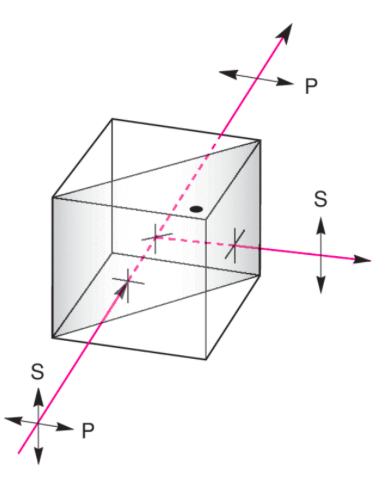
\includegraphics[width=4cm]{PBSC.png}
  \caption{Schematische Darstellung der Funktionsweise eines PBSC \cite{online1}}
  \label{fig:PBSC}
\end{figure}
Die Strahlen werden dann über drei weitere Spiegel weitergeleitet und bilden ein Rechteck, welches
sie in entgegengesetzer Richtung zueinander durchlaufen. Am Ende treffen sie wieder auf den
PBSC, wo sie jedoch keine Interferenzeffekte zeigen, da die Strahlen senkrecht zueinander polarisiert sind.
Hinter dem PBSC durchlaufen die sie dann entweder einen Polarisationsfilter der die beiden
Polarisationsrichtungen auf eine gemeinsame Achse projeziert, oder auf einen weiteren PBSC
welcher jedoch um $\SI{45}{\degree}$ in der Horizontalen gedreht ist,
sodass daraufhin in beiden Fällen Interferenzeffekte auftreten.\\
Zur Durchführung muss der Strahlengang zunächst mithilfe zweier Justageplatten so justiert werden,
dass die Strahlen nach dem zweiten Durchlaufen des PBSC möglichst überlappend und parallel laufen.
Um Interferenzeffekte beobachten zu können wird der zweite um 45° verkippte
Polarisationsfilter hinter den PBSC in den
Strahlengang eingebaut, sodass nun Interfernzstreifen zu erkennen sind.
Dies liegt daran, dass die zunächst senkrecht zueinander stehenden Strahlen durch den
Polarisationsfilter auf eine gemeinsame Achse projeziert werden und es zu Interferenzeffekten
in Abhängigkeit der Phasendifferenz kommt.
Da die Strahlen jedoch nicht komplett übereinander liegen, kommt es zu räumlichen Koherenzeffekten
und somit zu einem Strahlenmuster, welches sich durch Feinjustage der Spiegel verbreitert lässt.
Durch die Verbreiterung liegen die Streifen weit auseinander und die Photodiode kann
die Minima und Maxima besser trennen.\\
Nach der Feinjustage wird der Spiegel M2 verfahren, um den Strahl parallel zur ersten Oberfläche des PBSC zu bewegen.
Somit wird
der zuvor überlappende Strahlengang in zwei horizontal versetzte Strahlen aufgeteilt, was die getrennte
Manipluation eines der beiden Strahlen ermöglicht. Zudem
wird ein Rotationshalter mit 2 verkippten, jeweils $\SI{1}{\milli\metre}$ dicken Glasplatten
in den Strahlengang eingebaut.
Nach diesem Schritt wird noch einmal nachjustiert um
das Interferenzmuster möglichst zu verbreitern.\\
Zur Messung des Kontrastes in Abhängigkeit des Polarisationswinkels $\Phi$ des ersten
Polarisationsfilters hinter dem Laser wird die Intensität hinter dem zweiten
Polarisationsfilter und dem zweiten PBSC mithilfe einer Photodiode vermessen. Dabei werden für den Winkelbereich von
0° bis 180° in 5° bis 15° Schritten jeweils einmal die maximale und die minimale Intensität vermessen. Um dabei
zwischen konstruktiver und destruktiver Interferenz zu wechseln wird der Rotationshalter mit den Glasplatten
etwas gedreht. \\
Für die weiteren Messungen wird der zweite Polarisationsfilter entfernt und die beiden von
dem zweiten PBSC aufgespalteteten Strahlen werden mit zwei unterschiedlichen
Photodioden detektiert. Dies erlaubt das Auslesen über die Differenzspannungsmethode,
sodass die Messung nicht von möglichen Schwankungen der Laserintensität beeinflusst wird.
Der Polarisationsfilter wird dabei so eingestellt,
dass der Kontrast maximal ist. Die Anzahl der Maxima und Minima wird mithilfe eines
Modern Interferometry Controllers detektiert, wobei das Signal zusätzlich auf einem
Oszilloskop dargestellt wird. \\
Zur Bestimmung des Brechungsindex von Glas wird die Anzahl der Maxima und Minima
der Intensität beim Drehen von -4° bis 7° gemessen. Dieser Vorgang wird insgesamt 10 mal wiederholt.
\\
Anschließend wir zusätzlich eine Gaszelle der Länge $L=\SI{100}{\milli\metre}$
in den Strahlengang einer der beiden versetzten Strahlen
eingebaut, die mithilfe einer Pumpe zunächst evakuiert wird. Der Druck lässt sich dabei
über ein Druckmessgerät ablesen.
In die Zelle wird dann wieder kontrolliert Luft eingeleitet, wobei in Schritten
von $\SI{50}{\milli\bar}$ die Anzahl der Interferenz Minima und Maxima notiert wird. Dieser
Messprozess wird insgesamt drei mal durchgeführt.
